\section{Discussion and conclusions}
\label{sec:results}

\subsection{Discussion of results}


As detailed above, this research aimed to establish a reliable model for classifying tissue section images. Initially, simple CNN models were implemented, but upon observing limited success, the study shifted towards image preprocessing and finally settled on transfer learning with the InceptionV3 model, which produced the best results.

It is worth noting that with the trial of different models, as the model parameters are adjusted or the model architecture becomes more complex (such as InceptionV3), the model's performance significantly improves, i.e., the accuracy of the validation set becomes higher and the loss becomes lower.

Furthermore, comparing model series 1 and 2, we found that using preprocessed images to assist the machine in extracting features is not very effective in the task of image classification. Image processing may lead to the loss of important details and information, thereby affecting the machine's feature extraction, and thus affecting the accuracy and performance of the model.

In Section 5, we tested the model in application. First, we selected an additional test set to test the model's accuracy and found that the model's accuracy on all test sets was greater than 85\%. Then we used the model to evaluate different cutting angles and found that if the cutting quality is to be guaranteed at 80\%, the cutting angle should be between 9 degrees and 10.5 degrees. Finally, we used another dataset of fish alveolar slice images for secondary verification and found that the model's prediction accuracy for the test set labels was all above 90\%, reflecting that the model can be well applied to other datasets.

The Final selected model configuration, illustrated below, highlights the structured approach taken to integrate the InceptionV3 architecture effectively within the training framework.

\begin{center}

    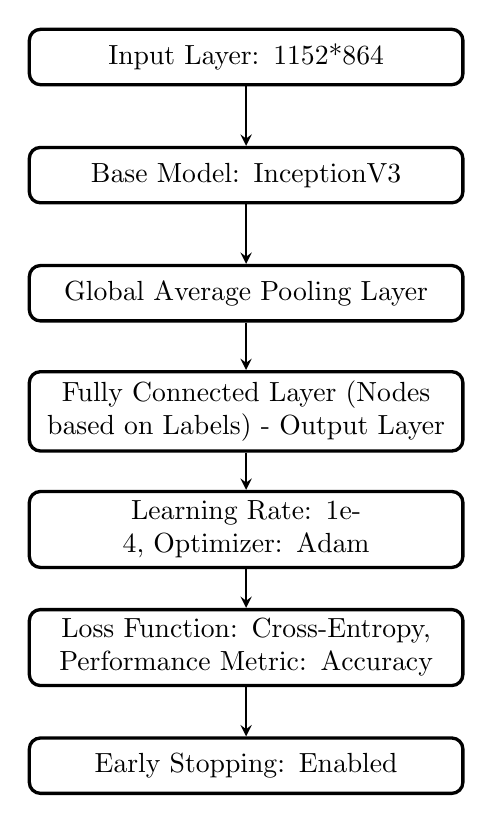
\begin{tikzpicture}[node distance=1.5cm,
        box/.style={
            rectangle,
            rounded corners,
            draw=black, very thick,
            text width=15em,
            minimum height=2em,
            text centered},
        arrow/.style={
            thick,
            ->,
            >=stealth}
        ]
    
        \node (collect) [box] {Input Layer: 1152*864};
        \node (mix) [box, below of=collect] {Base Model: InceptionV3};
        \node (train) [box, below of=mix] {Global Average Pooling Layer};
        \node (test) [box, below of=train] {Fully Connected Layer (Nodes based on Labels) - Output Layer};
        \node (evaluate) [box, below of=test] {Learning Rate: 1e-4, Optimizer: Adam};
        \node (rate) [box, below of=evaluate] {Loss Function: Cross-Entropy, Performance Metric: Accuracy};
        \node (improve) [box, below of=rate] {Early Stopping: Enabled};
        
        \draw [arrow] (collect) -- (mix);
        \draw [arrow] (mix) -- (train);
        \draw [arrow] (train) -- (test);
        \draw [arrow] (test) -- (evaluate);
        \draw [arrow] (evaluate) -- (rate);
        \draw [arrow] (rate) -- (improve);
        
        \end{tikzpicture}
\end{center}

\subsection{Future work}

\subsubsection{Enhancing Classification Methods}

\textbf{Broadening Classification Categories}

The current research has demonstrated promising results with the classification methods employed; however, the scope of classification remains limited to five categories. Enhancing the diversity of these categories could facilitate a deeper understanding of the relationships between cutting angles and sample quality, providing more precise analytical capabilities. More comprehensive classification could enable the prediction of optimal cutting angles based on a wider range of tissue responses, potentially improving outcomes for various tissue types and conditions.

\textbf{Transitioning to Linear Analytical Methods}

With a sufficiently granular set of classification points, it may become feasible to transition from a categorical framework to linear analytical methods. When enough categories are present, these can be approximated as discrete points within a linear relationship, allowing for linear regression to model the relationship between cutting angles and sample quality.

Linear Discriminant Analysis (LDA) is a statistical method used when categorical outcomes can be linearized, as discussed in the context of cutting angles. Employing LDA, especially in determining optimal cutting angles, could provide a more refined approach to correlating tissue quality with cutting parameters. This method could simplify the prediction of cutting parameters and aid in more precisely controlling the tissue sectioning process.

\textbf{Challenges and Considerations}

Transitioning from a classification problem to a linear discriminant analysis framework is challenging. One significant issue is that while binary classification models output probabilities, linear regression inherently seeks to identify relationships between variables (e.g., cutting angles as independent variables and cutting quality as the dependent variable). Moreover, the relationship between cutting angles and tissue quality is likely not a simple linear one, complicating the data the model needs to handle.

Further, training and validating linear models require significantly more data, potentially several orders of magnitude greater than currently used, making data collection a lengthy and challenging process. In addition, training and validating linear regression models demand substantial computational resources. Currently, using the TensorFlow framework with an InceptionV3 model at an input resolution of 1152x864 is pushing the limits of available GPU memory, suggesting that advancements in this area require additional hardware and computational power.

\textbf{Long-term Goals and Resource Needs}

These improvements represent long-term goals needing considerable resources and time. Research into linear discriminant analysis, for instance, involves deeper theoretical exploration and practical testing. For example, Jie Wen's work on "Robust Sparse Linear Discriminant Analysis" introduces sparsity into the LDA framework, making the model more robust and potentially more suited to complex real-world applications\cite{6.1}.


% (如果可以增加相关论文证明观点:二分类和线性回归问题的对比和性能开销)


\subsubsection{Performance Enhancement and Optimization}

As this research progresses towards large-scale application, performance optimization emerges as a crucial challenge. This involves not only enhancing algorithm efficiency but also improving the scalability, stability, and deployment capabilities of the model framework, as well as optimizing the underlying programming languages and code.

To optimize the use of computational resources, adopting more efficient computing frameworks and parallel processing algorithms is essential. Utilizing distributed computing resources can significantly reduce model training times and enhance efficiency when processing large datasets. Moreover, considering constraints on energy consumption and computational costs, it's vital to optimize the model's computational architecture and parameter settings to maximize output within limited resources.

The article "Analysis of the Application Efficiency of TensorFlow and PyTorch in Convolutional Neural Network" highlights the differences between TensorFlow and PyTorch in processing convolutional neural networks\cite{6.2}. TensorFlow exhibits a lower error rate and smaller convergence steps, whereas PyTorch offers faster training speeds.

Pascal Fua's "Comparing Python, Go, and C++ on the N-Queens Problem" presents methods to optimize deep learning performance by comparing the efficiency of Python, Go, and C++ in solving the N-Queens problem.\cite{6.3} It was found that runtime languages have clear advantages in handling loops and data flows, suggesting that compiling tools like Numba, Cython, and Pybind11 can enhance performance in deep learning applications.

% (论文:tf和torch的对比,libtf libtf,opencv c++和py的对比)

\subsubsection{Optimization of the Sectioning Process}

Our research also uncovered that real-time assessment of section quality during the cutting process, followed by adjustments based on those assessments, could significantly improve the quality of tissue sections.

The proposed feedback adjustment process involves installing a camera above the microtome to capture data from the samples being cut. This data is then analyzed in real-time by a pre-trained model, which assesses the quality of the sections. Based on this assessment, the cutting speed and angle parameters of the microtome can be adjusted to improve the quality of subsequent sections, thus ensuring controllable and consistent sample quality.

Implementing this system presents several challenges:

\begin{itemize}
    \item \textbf{Real-Time Image Processing:} A clear camera and an efficient real-time image processing system are needed to capture and process image data swiftly.
    \item \textbf{Powerful Computing Resources:} A pre-trained model and a powerful computer are required to quickly assess images and adjust the microtome's parameters based on the assessment.
    \item \textbf{Effective Control Interface:} An efficient control interface is necessary to ensure that the adjusted parameters are promptly communicated to the microtome.
    \item \textbf{Time Efficiency:} The entire system must operate within the brief intervals between cuts.
\end{itemize}

A pertinent example can be found in the study "Convolutional neural networks applied to microtomy: Identifying the trimming-end cutting routine on paraffin-embedded tissue blocks"\cite{6.4}. This research automated the sectioning process by monitoring it with a camera, analyzing the images with a CNN, and adjusting the microtome parameters based on the analysis. This integration of the microtome, camera, and deep learning model provides a feasible solution for real-time assessment and adjustment of cutting parameters during the sectioning process.


\subsection{Conclusions}

This research has significantly advanced our understanding of optimizing biopsy parameters through the application of deep learning techniques to biomedical tissue sectioning devices. By employing sophisticated convolutional neural networks, particularly through the adaptation of the InceptionV3 model via transfer learning, the study has demonstrated a robust framework capable of assessing the quality of tissue sections with high precision. This approach not only improves the accuracy of tissue sample analysis but also introduces a paradigm shift in the operational methodology of tissue sectioning.

By evaluating the quality of sections at different angles, we have discovered the relationship between the cutting angle and the quality of the sections. This provides us with a feasible method to improve the quality of sections in the future. In addition, the application of this model in different types of tissues (including fish ovaries and lung tissues) has confirmed its wide adaptability and potential for promotion, indicating that it is suitable for various tissue sections and research tasks.

However, the study also highlighted the limitations of traditional image preprocessing techniques. Initial attempts to enhance model performance through image preprocessing did not yield significant improvements and, in some cases, potentially obscured critical details necessary for accurate classification. This finding suggests that maintaining the integrity of original image data might be more beneficial than applying aggressive preprocessing techniques.

The research also explored the possibility of real-time assessment and automatic adjustment of sectioning parameters, proposing a feedback system that integrates image capture, real-time analysis, and mechanical adjustment to enhance the quality of sections dynamically. This system points towards the future of automated histology instruments, which could significantly reduce human error and variability in tissue sectioning.

In conclusion, this project not only demonstrates the important role of deep learning in biomedical research and applications, but also provides feasibility for the further improvement of tissue sectioning technology. The combination of these technologies can bring improvements to biological sectioning equipment, provide a possible solution to improve the yield rate of tissue samples and the efficiency of sectioning. This research provides new ideas and methods for future tissue sectioning technology, and is expected to have a profound impact in the field of biomedicine.

% 总之,该项目不仅体现了深度学习在生物医学研究和应用中的重要作用,而且为组织切片技术的进一步提高提供了可行性。将这些技术的有机结合能够为生物切片设备带来改进,提高组织样本的良品率及提高切片效率提供了一个可能的解决方案。这一研究为未来的组织切片技术提供了新的思路和方法,有望在生物医学领域产生深远的影响。

\FloatBarrier % Now the table doesn't flow over to any other sections